\documentclass[sigplan,screen]{acmart}

\usepackage{booktabs} % For formal tables
\usepackage{balance}
\usepackage{multirow}
\usepackage{listings}

\usepackage{tikz}
\usetikzlibrary{automata,positioning}

\usepackage{balance}

\makeatletter
    \def\balanceissued{unbalanced}%flag to indicate if \balance has been used
    \let\oldbibitem\bibitem
    \def\bibitem{%
            \expandafter\ifx\expandafter\relax\balanceissued\relax\else%
                \balance%
                \gdef\balanceissued{\relax}\fi%
        \oldbibitem}
\makeatother

\lstset{
  frame=none,
  language=scala,
  basicstyle={\footnotesize\ttfamily},
  showspaces=true
}

\makeatletter
\def\lst@visiblespace{ }
\makeatother

\sloppy

\clubpenalty = 10000
\widowpenalty = 10000
\displaywidowpenalty = 10000

% DOI
%\acmDOI{10.475/123_4}

% ISBN
%\acmISBN{123-4567-24-567/08/06}

%Conference
%\acmConference[Scala 2018]{Ninth ACM SIGPLAN Symposium on Scala, 2018}{September 2018}{St. Louis, Missouri, United States}
%\acmYear{2018}
%\copyrightyear{2018}

%%% If you see 'ACMUNKNOWN' in the 'setcopyright' statement below,
%%% please first submit your publishing-rights agreement with ACM (follow link on submission page).
%%% Then please update our instructions page and copy-and-paste the NEW commands into your article.
%%% Please contact us in case of questions; allow up to 10 min for the system to propagate the information.
%%%
%%% The following is specific to Scala '18 and the paper
%%% 'Parser Combinators for Context-Free Path Querying'
%%% by Ekaterina Verbitskaia, Ilya Kirillov, Ilya Nozkin, and Semyon Grigorev.
%%%
\copyrightyear{2018}
\acmYear{2018}
\setcopyright{acmcopyright}
\acmConference[Scala '18]{Proceedings of the 9th ACM SIGPLAN International Scala Symposium}{September 28, 2018}{St. Louis, MO, USA}
\acmBooktitle{Proceedings of the 9th ACM SIGPLAN International Scala Symposium (Scala '18), September 28, 2018, St. Louis, MO, USA}
\acmPrice{15.00}
\acmDOI{10.1145/3241653.3241655}
\acmISBN{978-1-4503-5836-1/18/09}

%\acmArticle{4}
%\acmPrice{15.00}

% These commands are optional
%\acmBooktitle{Transactions of the ACM Woodstock conference}
%\editor{Jennifer B. Sartor}
%\editor{Theo D'Hondt}
%\editor{Wolfgang De Meuter}

\citestyle{acmauthoryear}


\begin{document}
\title{Parser Combinators for Context-Free Path Querying}
%\titlenote{This work is supported by grant from JetBrains Research.}
%\subtitle{Extended Abstract}
%\subtitlenote{The full version of the author's guide is available as
%  \texttt{acmart.pdf} document}


\author{Ekaterina Verbitskaia}
\affiliation{%
  \institution{Saint Petersburg State University}
  \streetaddress{7/9 Universitetskaya nab.}
  \city{St. Petersburg}
  \country{Russia}
  \postcode{199034}
}
\email{kajigor@gmail.com}

\author{Ilya Kirillov}
\affiliation{%
  \institution{Saint Petersburg State University}
  \streetaddress{7/9 Universitetskaya nab.}
  \city{St. Petersburg}
  \country{Russia}
  \postcode{199034}
}
\email{kirillov.ilija@gmail.com}

\author{Ilya Nozkin}
\affiliation{%
  \institution{Saint Petersburg State University}
  \streetaddress{7/9 Universitetskaya nab.}
  \city{St. Petersburg}
  \country{Russia}
  \postcode{199034}
}
\email{nozhkin.ii@gmail.com}


\author{Semyon Grigorev}
\orcid{0000-0002-7966-0698}
\affiliation{%
  \institution{Saint Petersburg State University}
  \streetaddress{7/9 Universitetskaya nab.}
  \city{St. Petersburg}
  \country{Russia}
  \postcode{199034}
}
\email{s.v.grigoriev@spbu.ru}

% The default list of authors is too long for headers.
\renewcommand{\shortauthors}{Verbitskaia et al.}

\begin{abstract}
Transparent integration of a domain-specific language for specification of context-free path queries (CFPQs) into a general-purpose programming language as well as static checking of errors in queries may greatly simplify the development of applications using CFPQs.
LINQ and ORM can be used for the integration, but they have issues with flexibility: query decomposition and reusing of subqueries are a challenge.
Adaptation of parser combinators technique for paths querying may solve these problems.
Conventional parser combinators process linear input, and only the Trails library is known to apply this technique for path querying.
Trails suffers the common parser combinators issue: it does not support left-recursive grammars and also experiences problems in cycles handling.
We demonstrate that it is possible to create general parser combinators for CFPQ which support arbitrary context-free grammars and arbitrary input graphs.
We implement a library of such parser combinators and show that it is applicable for realistic tasks.
\end{abstract}

%
% The code below should be generated by the tool at
% http://dl.acm.org/ccs.cfm
% Please copy and paste the code instead of the example below.
%
\begin{CCSXML}
<ccs2012>
<concept>
<concept_id>10002951.10002952.10002953.10010146</concept_id>
<concept_desc>Information systems~Graph-based database models</concept_desc>
<concept_significance>500</concept_significance>
</concept>
<concept>
<concept_id>10002951.10002952.10003197.10010825</concept_id>
<concept_desc>Information systems~Query languages for non-relational engines</concept_desc>
<concept_significance>500</concept_significance>
</concept>
<concept>
<concept_id>10011007.10011006.10011008.10011009.10011012</concept_id>
<concept_desc>Software and its engineering~Functional languages</concept_desc>
<concept_significance>300</concept_significance>
</concept>
<concept>
<concept_id>10003752.10003766.10003771</concept_id>
<concept_desc>Theory of computation~Grammars and context-free languages</concept_desc>
<concept_significance>300</concept_significance>
</concept>
</ccs2012>
\end{CCSXML}

\ccsdesc[500]{Information systems~Graph-based database models}
\ccsdesc[500]{Information systems~Query languages for non-relational engines}
\ccsdesc[300]{Software and its engineering~Functional languages}
\ccsdesc[300]{Theory of computation~Grammars and context-free languages}

\keywords{Graph Databases, Language-Constrained Path Problem, Context-Free Path Querying, Context-Free Language Reachability, Parser Combinators, Generalized LL, GLL, Neo4j, Scala}

\maketitle

\section{Introduction}

Graph querying is finding all paths in the graph which satisfy some constraints.
If the constraints are specified with some language formalism, i.e. a grammar, it is called a language-constrained path query. The simplest query described with a grammar $S \rightarrow a \ b$ being run against the graph in the Fig.~\ref{fig:exmplInputGraph} returns the only path $2, 3, 4$ (shown in red).

A grammar $S \rightarrow a \ S \ b \mid a \ b$ is a query for the paths of the form $a^n b^n$, where $n \geq 1$.
Querying the graph in the Fig.~\ref{fig:exmplInputGraph} returns the infinite set of paths one of which starts and ends in the vertex $3$ and goes around the cycles in the graph the appropriate number of times: $3,1,2,3,1,2,3,4,3,4,3,4,3$.

\begin{figure}[h]
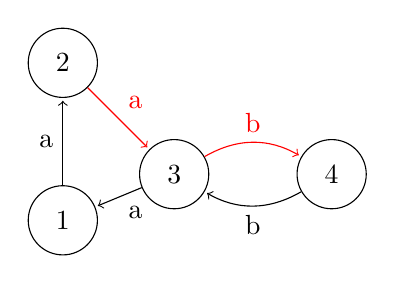
\begin{tikzpicture}[shorten >=1pt,node distance=2cm,on grid,auto]
   \node[state] (q_1)   {$1$};
   \node[state] (q_2) [above=of q_1] {$2$};
   \node[state] (q_3) [above right=of q_1, below right=of q_2] {$3$};
   \node[state] (q_4) [right=of q_3] {$4$};
    \path[->]
    (q_1) edge  node {a} (q_2)
    (q_2) edge[red]  node {a} (q_3)
    (q_3) edge  node {a} (q_1)
    (q_3) edge[bend left, above, red]  node {b} (q_4)
    (q_4) edge[bend left, below]  node {b} (q_3);
\end{tikzpicture}
\caption{An example of input graph}
\label{fig:exmplInputGraph}
\end{figure}

Most existing graph traversing/querying languages, including SPARQL~\cite{sparql}, Cypher~\footnote{Cypher language web page: \url{https://neo4j.com/developer/cypher-query-language/}. Access date: 16.01.2018}, and Gremlin~\cite{gremlin} support only regular languages as constrains.
For some applications, regular languages are not expressive enough.
Context-free path queries (CFPQ), on which we focus this paper, employ context-free languages for constraints specification.
CFPQs are used in bioinformatics~\cite{GraphQueryWithEarley}, static code analysis~\cite{Reps, Zheng, LabelFlowCFLReachability, specificationCFLReachability, JavaCFL}, and RDF processing~\cite{CFGonRDF}.
Although there is a lot of problem-specific solutions and theoretical research on CFPQs~\cite{Yannakakis, ConjCFPathQuery, Hellings16, GrigorevR16, QueryGraphWithData, RegularDBQuery, GraphQueryWithEarley, graphDB}, cfSPARQL~\cite{CFGonRDF} is the single known graph query language to support CF constraints.
Generic solution for the integration of CFPQs into general-purpose languages is not discussed enough.

When developing a data-centric application, one wants to use a general-purpose programming language and also to have transparent and native access to data sources.
One way to achieve this is to use string-embedded DSLs.
In this approach, a query is written as a string, then passed on to a dedicated driver which executes it and returns a possibly untyped result.
Despite the simplicity, string-embedded DSLs have serious drawbacks.
First of all, they require the developer to learn the language itself, its features, runtime, and how the integration between the languages is implemented.
DSLs are also a source of possible errors and vulnerabilities, static detection of which is a serious challenge~\cite{stringEmbeddedLanguagesProblem}.
Such techniques as the Object Relationship Mapping (ORM) or Language Integrated Query~(LINQ)~\cite{LINQ1, LINQ2, LinqRDF} partially solve these problems, but they still have issues with flexibility: both query decomposition and  reusing of subqueries are a struggle.
In this paper, we propose a transparent and natural integration of CFPQs into a general-purpose programming language.

Context-free path queries are known in various domains under different names. The \emph{context-free language reachability framework} or  \emph{IFDS framework} is how they are called in the area of static code analysis.
In~\cite{Reps:1995, Reps} Thomas Reps shows that the wide range of static code analysis problems can be formulated in terms of CFL-reachability in the graph.
This framework is used for such problems as the taint analysis~\cite{CFLTaint}, the alias analysis~\cite{JavaCFL, Zheng, CFLGraspan}, the label flow analysis~\cite{LabelFlowCFLReachability}, and the fix locations problem~\cite{CFLfinding}.
What we propose in the paper can be viewed as a core of such framework since it provides both problem and domain independent mechanism for CFPQ evaluation.

We view parser combinators as the best way to integrate context-free language specifications into a general-purpose programming language. Parser combinators provide not only a transparent integration but also compile-time checks of correctness and high-level techniques for generalization. An idea to use combinators for graph traversing has already been proposed in~\cite{ScalaGraphParsing}. Unfortunately, the solution presented processes cycles in the input graph only approximately and is unable to handle left-recursive combinators, which is the most common issue of the approach. Authors pointed out that the idea described is similar to the parser combinators, but the language class supported or restrictions are not discussed.

Parser combinators are known to handle only a subset of context-free grammars: left recursion and ambiguity of the grammars are problematic.
In~\cite{Meerkat}, the authors demonstrate a set of parser combinators which handles arbitrary context-free grammars by using ideas of the Generalized LL~\cite{scott2010gll} algorithm (GLL).
Meerkat~\footnote{Meerkat project repository:~\url{https://github.com/meerkat-parser/Meerkat}. Access date: 16.01.2018} parser combinators library implements the ideas from the paper~\cite{Meerkat} and provides the parsing result in a compact form as a Shared Packed Parse Forest~\cite{SPPF}~(SPPF).
SPPF is a suitable finite structural representation of a CFPQ result, even when the set of paths is infinite~\cite{GrigorevR16}.
All the paths can be extracted from the SPPF---in the form of the corresponding derivation trees---and further analysis can be done.
It is also possible to run some further processing over the SPPF itself---not extracting the paths explicitly.

In this paper, we compose these ideas and present a set of parser combinators for context-free path querying which handles arbitrary context-free grammars and provides a structural representation of the result.
We make the following contributions in the paper.

\begin{enumerate}
\item We show that it is possible to create a set of parser combinators for context-free path querying which works on both arbitrary context-free grammars and arbitrary graphs and provides a finite structural representation of the query result.
\item We implement the parser combinators library in Scala. This library provides integration to Neo4j~\footnote{Neo4j graph database site: \url{https://neo4j.com/}. Access date: 16.01.2018} graph database. The source code is available on GitHub: \url{https://github.com/YaccConstructor/Meerkat}.
\item We perform an evaluation on realistic data and compare the performance of our library with another GLL-based CFPQ tool and with the Trails library.
We conclude that our solution is expressive and performant enough to be applied to the real-world problems.
\end{enumerate}

This paper is organized as follows.
We introduce a formal definition of the CFPQ problem in section~\ref{sec:CFPQ}, and we provide a basic description of the Meerkat library and SPPF data structure in section~\ref{sec:GLL}.
We describe our solution in section~\ref{sec:combinators}.
In section~\ref{sec:examples} we present and discuss a set of classical queries (the same generation query, the queries to a movie dataset~\footnote{The movie database is a traditional dataset for graph databases. Detailed description is available here: \url{https://neo4j.com/developer/movie-database/}. Access date: 16.01.2018})
written with our library.
Evaluation of the library is described in section~\ref{sec:evaluation}.
Finally, In section~\ref{sec:conclusion} we conclude and discuss possible directions for further research.

\section{Context-Free Path Querying Problem}
\label{sec:CFPQ}

In this section, we formally describe the context-free path querying problem and the context-free reachability problem.

First, we introduce the necessary definitions.
\begin{itemize}
  \item A context-free grammar is a quadruple $G=(N, \Sigma, P, S)$, where $N$ is a set of nonterminal symbols, $\Sigma$ is a set of terminal symbols, $S \in N$ is a start nonterminal, and $P$ is a set of productions.
  \item $\mathcal{L}(G)$ denotes a language specified by the grammar $G$, and is a set of terminal strings derived from the start nonterminal of $G$: $\mathcal{L}(G) = \{\omega \mid S \Rightarrow_{G}^{*} \omega\}$.
  \item A directed graph is a triple $M = (V,E,L)$, where $V$ is a set of vertices, $L \subseteq \Sigma$ is a set of labels, and a set of edges $E\subseteq V\times L\times V$.
  Note that there are not parallel edges with equal labels: if $(v, l_1, u) \in E$ and $(v,l_2,u) \in E$, then $l_1 \neq l_2$.
  \item $tag: E \rightarrow L$ is a function which returns a tag of an edge. $$tag((\_,l,\_)) = l$$
  \item $\oplus: L^+ \times L^+ \rightarrow L^+$ denotes a tag concatenation operation.
  \item $\Omega$ is a helper function which constructs a string produced by the given path. For every $p \text{ path in } M$
  $$ \Omega(p = e_{0},e_{1},\dots,e_{n-1}) = tag (e_{0}) \oplus \dots \oplus tag (e_{n-1}).$$
\end{itemize}

We define the context-free language constrained path querying as, given a query in the form of a grammar $G$, to construct the set of the paths from the input graph $M$ which are also strings derivable in the grammar $G$: $$\{p \mid p \text{ is a path in } M, \Omega(p) \in \mathcal{L}(G)\}.$$
The CFL reachability problem is pretty similar, but here one is only concerned with the existence of the paths derived by the grammar. It is formulated as follows:
$$\{ (v_0,v_n) \mid p \text{ is a path in } M, \Omega(p) \in \mathcal{L}(G),$$
$$p = v_0 \rightarrow \cdots \rightarrow v_n\}.$$

Note that the query result can be an infinite set, hence it cannot be represented explicitly.
We show how to construct a compact data structure which stores all the elements of the query result in a finite space; every path can be extracted from this representation.
\section{Generalized Parser Combinators}
\label{sec:GLL}

Combinators techniques are shown to be applicable for graph traversing~\cite{ScalaGraphParsing}, but it still suffers from the common issue with left-recursive definitions.
A general parser combinators library Meerkat~\cite{Meerkat}, implemented in the Scala programming language, removes this restriction by using memoization, continuation-passing style, and the ideas of Johnson~\cite{Johnson}.
Meerkat converts parsers into a memoized versions of themselves.
The memoization routine stores parsing results the first time they are computed and reuses them every time they are needed again.
Every time a new parsing result for some combinator is calculated, all the combinators, which are dependent on it, are recomputed.
This way Meerkat employs left-recursive parser combinators, and it is also crucial for the handling of the cycles in the input graphs.

Meerkat supports the arbitrary (left-recursive and ambiguous) context-free specifications; it also supports the specification of action codes and provides a \lstinline{syn} macro for custom handling of the recursive nonterminal descriptions.
Meerkat constructs the compact representation of the parse forest in the form of SPPF, which can be used for CFPQs results representation~\cite{GrigorevR16}.
The worst case time and space complexity of the solution are cubic.

A Meerkat specification of the language $\{a^n b^n \mid n \geq 1\}$ is \lstinline{val S = syn("a" ~ S.? ~ "b")}. Here \lstinline{syn} is a macro which creates a parser: for example, it transforms string literals into parsers for those strings. The tilde \lstinline{~} stands for a sequential parser combinator, and the question mark \lstinline{?} describes optional parsing. Other combinators available in the Meerkat library are shown in Table~\ref{table:combinators}.

It is shown in~\cite{GrigorevR16} that the Generalized LL parsing algorithm~\cite{scott2010gll} can be generalized to process CFPQs effectively and the query result can be finitely represented.
As the Meerkat library is closely related to the Generalized LL algorithm, it is also possible to adapt the Meerkat library for graph querying.
It can be done by providing a function for retrieving the symbols which follow the specified position and utilizing it in the basic set of combinators.
Details are described in the next section.

\subsection{SPPF}

Parsing of a string with respect to an ambiguous grammar can result in several derivation trees for a single string.
The set of derivation trees is named a \emph{derivation forest}.
To store a derivation forest efficiently, the generalized parsing algorithms utilize a \emph{Shared Packed Parse Forest} proposed by Joan Rekers~\cite{SPPF}.
The most efficient compact representation of derivation forests is a Binarized Shared Packed Parse Forest (we will abbreviate it to SPPF)~\cite{brnglr}.
The GLL algorithm, which employs this structure, achieves the worst-case cubic space complexity~\cite{gllParsingTree}.

Binarized SPPF is a directed graph, each node of which has one of the four types described below.
Almost every node of the SPPF is decorated with the \emph{extension}: a pair $(i, j)$ where $i$ is a start position of a substring derivable from the node and $j$---its end position.

\begin{itemize}
    \item A \textbf{terminal node} is labelled $(T, i, j)$.
    \item A \textbf{nonterminal node} is labelled $(N, i, j)$.
    This node denotes that there is at least one derivation $N \Rightarrow^*_G \omega[i \dots j-1]$---a substring of the input from the $i$-th to the $j$-th position.
    Every derivation tree for the given substring and nonterminal can be extracted by left-to-right top-down traversal of SPPF started from the respective node.
    \item An \textbf{intermediate node}: a special kind of node used for the binarization of the SPPF. These nodes are labelled with $(t,i,j)$, where $t$ is a grammar slot.
    \item A \textbf{packed node} is labelled $(N \rightarrow \alpha, k)$, where $k$ is a position in the input of the right end of the leftmost subtree of this node.
    A subgraph with the root in such node is, in turn, a parse forest for which the first production is $N \rightarrow \alpha$.
\end{itemize}


An example of SPPF is presented in Fig.~\ref{fig:sppf}.
We removed redundant intermediate and packed nodes for simplicity and to decrease the size of the figure.

SPPF finitely represents a possibly infinite set of paths in the context of the language-constrained graph querying~\cite{GrigorevR16}.
Since the SPPF stores derivation trees for all paths, it is useful for postprocessing and further understanding of the query results.
In static code analysis, for example, it is possible to map paths back onto the source code thus providing a human-readable result.
\section{Parser Combinators for Path Querying}
\label{sec:combinators}

Parser combinators are a way to specify both a language syntax and a parser for it in terms of higher-order functions.
A parser in this framework is a function which consumes a prefix of input and returns either a parsing result or an error if the~input is erroneous.
Parser combinators compose parsers to form more complex parsers.
A parser combinators library usually provides a set of basic parser combinators, such as a combinator of the~sequential application or the~choice combinator, but there can also be user-defined combinators.
Most parser combinators libraries, including the~Meerkat library, can only process the~linear input---strings or streams.
We modify the~Meerkat library to work on the~graph input. The~following ideas are at the~core of the~modification.

The~intersection of a context-free and a regular language is context-free. There are several constructive proofs of this fact.
The~proposed solution is yet another constructive proof with the~SPPF as a user-friendly representation of the~context-free grammar for the~intersection.

Linear input can be regarded as a linear directed graph with symbols of the~input labelling the~edges.
A conventional parser moves a pointer in the~input from the~position $i$ to the~position $i+1$ and creates a new state when a token between the~$i$-th and the~$i+1$-th positions matches what is required in the~grammar.
In case of graph processing, there are possibly multiple ways to move from the~current vertex $i$, and it is possible to produce multiple new states.
Generalized parsing is designed to handle the~production of multiple new states optimally, thus it is suitable
 to handle graph processing.

Matching a token in the~input can be viewed as a predicate, for example, $p_c (x) = x == c$.
We can generalize this observation allowing matching of an edge label of an arbitrary type with a predicate of some sort.
If vertices of the~graph contain any data of interest, we can treat them in the~similar fashion as the~edges.
The~formal definition of the~context-free language constrained path querying changes only in a way a string is collected along a path in the~input graph: the~data stored in the~vertices should also be taken into consideration.

Handling cycles in the~input graphs imposes two challenges: not to get stuck in an infinite loop while processing the~positions and if a new parsing state appears at some position, all paths which pass through this state, should be accounted for.
The~Meerkat memoization routine solves both of these challenges.
Parsing from a parser state at each position is only run if it has never been run before, so since there is only a finite number of parsing states and positions in the~input, parsing terminates.
Appearing of the~new parsing state at a position which has been processed before triggers processing of every path possibly affected by it.
Thanks to the~memoization, each derivation of each subpath is analyzed only once, so there is no significant overhead at re-running.


Querying process in our library is inherited from generalized parsing and is done in two steps.
The~first step is ``parsing'': the~construction of the~SPPF which contains all derivation trees for the~paths satisfying syntactic constraints.
The second step is the application of semantic actions which retrieves the necessary additional data about the paths from the SPPF

\subsection{The~Set of Combinators}

In this section, we demonstrate the~set of combinators by example. The~input graph, which represents a map, is presented in Fig.~\ref{fig:graph}.
In the input graph, there are some cities connected by one-way roads depicted by the~edges labelled $road\_to$.
Each city is labelled by its name and a country it belongs to.

\begin{figure}[h]
\resizebox {0.45\textwidth} {!}
{
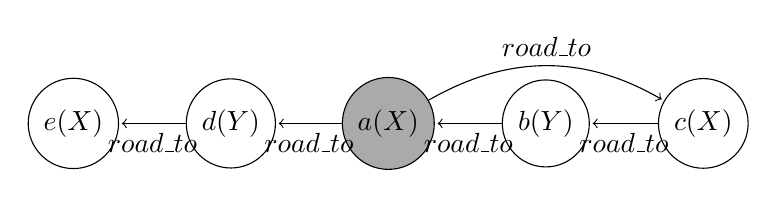
\begin{tikzpicture}[shorten >=1pt,node distance=2cm,on grid,auto]
   \node[state] (a) [fill={rgb:black,1;white,2}]  {$a(X)$};
   \node[state] (b) [right=of a] {$b (Y)$};
   \node[state] (c) [right=of b] {$c (X)$};
   \node[state] (d) [left=of a] {$d (Y)$};
   \node[state] (e) [left=of d] {$e (X)$};
    \path[->]
    (a) edge [bend left, above] node [above] {$road\_to$} (c)
    (b) edge  node {$road\_to$} (a)
    (c) edge  node {$road\_to$} (b)
    (a) edge  node {$road\_to$} (d)
    (d) edge  node {$road\_to$} (e);
\end{tikzpicture}
}
\caption{Example graph. Vertex labels are in the~form "city-name (country-name)"}
\label{fig:graph}
\end{figure}

Two basic building blocks of queries are the~combinators for dealing with edges and vertices.
\begin{itemize}
    \item \lstinline{V[N](predicate: N => Boolean)} the~combinator for processing vertices, where \lstinline{N} is a type of the~node label.
    Parsing with this combinator succeeds iff the~vertex satisfies the~predicate.
    \item \lstinline{E[L](predicate: L => Boolean)} the~combinator for processing edges, where \lstinline{L} is a type of the~edge label.
    Parsing with this combinator succeeds iff the~edge satisfies the~predicate.
\end{itemize}

\begin{figure}[t]
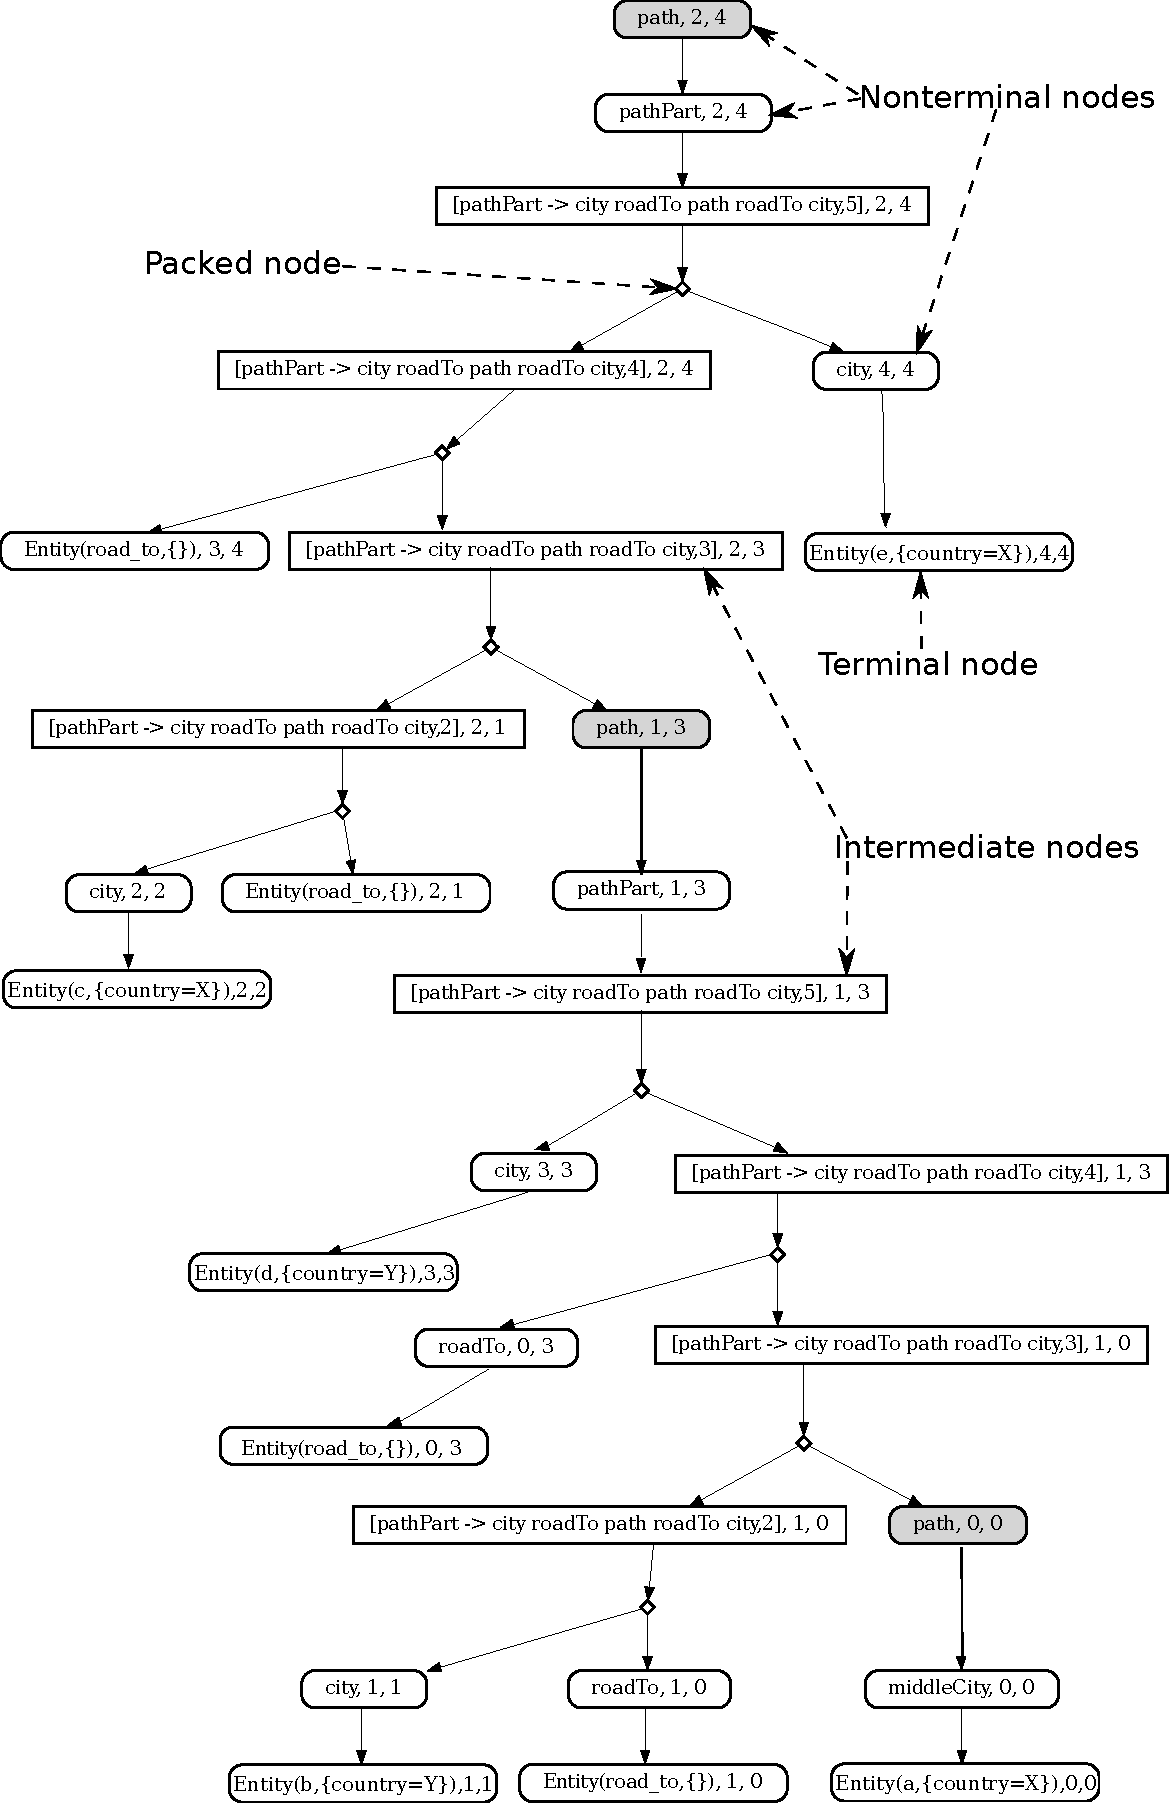
\includegraphics[width=\columnwidth]{sppf}
\caption{SPPF: result of applying cities query to the~graph~\ref{fig:graph}}
\label{fig:sppf}
\end{figure}

To select cities which belong to some country, we can use the~function \lstinline{V}: \lstinline{V[N]((e: Entity) => e.country = "County Name")}.
Here \lstinline{Entity} is a property container for both edges and vertices.
By using the~\lstinline{Dynamic} trait, all accesses to properties (like \lstinline{(e: Entity).country}) are converted to the~accesses to the~properties of either a vertex or an edge.
For the~sake of simplicity, we will omit \lstinline{Entity} type specifications for predicates.
To query the~graph for the~paths from a city in the~country $X$ to a city in the~country $Y$, we need to sequentially compose the~combinators for selecting the~appropriate cities.
A sequential combinator \lstinline{~} does just that: it sequentially  applies two queries one after the~other.
Let us denote a query for retrieving a city from the~specific country \lstinline{city(name: String)} and a query for retrieving road edges \lstinline{roadTo}.
With this denotation, a query \lstinline{city("X") ~ roadTo ~ city("Y")} returns the~requested set of paths from the~graph.
The~query with all necessary subqueries is the~following\footnote{Underscore in anonymous lambda functions serves as a placeholder for an argument: \lstinline{(_.country == country)} is equavalent to \lstinline{(x => x.country == country)} }.

\begin{lstlisting}
def city(country: String) = V(_.country == country)
val roadTo = E(_.value() == "road_to")
val ourPath = city("X") ~ roadTo ~ city("Y")
\end{lstlisting}

The~next step after writing the~query is to implement a function to retrieve the~actual data about the~paths.
If we care only about the~names of the~cities, we can return a pair of the~cities for each path.
First, we modify the~query for vertices by adding the~semantic action to it using the~combinator \lstinline{^}:

\begin{lstlisting}
def city(name: String) =
  syn(V(e.value() == name) ^ (_.value))}
\end{lstlisting}

Then we need to map a path to a pair of cities: this is done with the~combinator \lstinline{&}.
The~complete query returns the~sequence of pairs of cities which have the~road between them:

\begin{lstlisting}
def city(country: String) =
  syn(V(_.country() == country) ^ (_.name))
val roadTo = E(_.value() == "road_to")
val ourPath =
  syn(city("X") ~ roadTo ~ city("Y") &
    { case c0 ~ c1 => (c0, c1) })
\end{lstlisting}

The~whole set of basic combinators, which our library provides, is presented in Table~\ref{table:combinators}.
There are two kinds of combinators: the~first kind combines parsers to form new parsers; meanwhile the~second one is dedicated to the~processing of the~query result.
Whenever a string is used within a query, a parser which matches that string is generated implicitly.

\begin{table}[h]
\small
\centering
\caption{Basic combinators}
\label{table:combinators}
\begin{tabular}{l@{}|l}
\multicolumn{1}{c|}{Combinator} & \multicolumn{1}{|c}{Description} \\ \hline
{\lstinline!a ~ b!} & sequential parsing: {\lstinline!a!} then {\lstinline!b!}   \\
{\lstinline!a | b!} & choice: {\lstinline!a!} or {\lstinline!b!}         \\
{\lstinline!a ?!}   & optional parsing: {\lstinline!a!} or nothing   \\
{\lstinline!a *!}   & repetition of zero or more {\lstinline!a!} \\
{\lstinline!a +!}   & repetition of at least one {\lstinline!a!} \\
{\lstinline!a ^ f!} & apply {\lstinline!f!} function to {\lstinline!a!} if  {\lstinline!a!} is a token \\
{\lstinline!a ^^!}  & capture output of {\lstinline!a!} if {\lstinline!a!} is a token    \\
{\lstinline!a & f!} & apply {\lstinline!f!} function to {\lstinline!a!} if  {\lstinline!a!} is a parser \\
{\lstinline!a &&!}  & capture output of {\lstinline!a!} if {\lstinline!a!} is a parser    \\
\hline
\end{tabular}
\end{table}


\subsection{Generic Interface for Input}
The~combinators in our library are independent of the~input representation.
It is enough to specify two basic combinators which handle vertices and edges.
Vertex handling is checking whether the~vertex satisfies the~given predicate.
In case of the~edges, one needs to check which of the~edges outgoing from the~given vertex satisfy the~given predicate.
These two functions form the~trait for the~input (Fig.~\ref{fig:input}).
It has two type parameters: the~type of edge labels \lstinline{L} and the~type of vertices labels \lstinline{N}.
Since the~required functions are simple, we believe it is possible to support most storages of graph-structured data.
We supported several different input sources:

\begin{itemize}
    \item Neo4jInput: input source for the~graph database Neo4j;
    \item GraphxInput: input source for the~graph presented in memory using the~GraphX library;
    \item LinearInput: input source for the~linear input data such as the~ordinary strings.
\end{itemize}

\begin{figure}[t]
\begin{lstlisting}
trait Input[+L, +N] {
  def filterEdges(nodeId: Int,
      predicate: L => Boolean): Seq[(L, Int)]
  def checkNode(nodeId: Int,
      predicate: N => Boolean): Option[N] }
\end{lstlisting}
\caption{Generalized input interface}
\label{fig:input}
\end{figure}

\subsection{Semantic Actions}
\label{sec:semanticActions}

Every path, which the~query produces, has a derivation tree stored in the~SPPF.
The~derivation tree is a very rich data structure which can be hard to understand.
The~library provides a mechanism of semantic actions to retrieve the~data useful for the~user.
It is a way to apply some function to a parsed token or a subsequence.

Semantic action binder for the~tokens---vertices and edges alike---is \lstinline{^}. The~most common use for it is to extract properties from the~token and combine them in some fashion.

\begin{lstlisting}
// Defined in Terminal[+L] (edge) parser
def ^[U](f: L => U) =
  new SymbolWithAction[L, Nothing, U] {...

// Defined in Vertex[+N] parser
def ^[U](f: N => U) =
  new SymbolWithAction[Nothing, N, U] {...
\end{lstlisting}

For the~combination of parsers, there is a \lstinline{&} binder. Being  applied to a sequence of tokens, it can collect and process the~data returned by the~terminal parsers.

\begin{lstlisting}
// Defined in Symbol[+L, +N, +V] parser
def &[U](f: V => U) =
  new SymbolWithAction[L, N, U] {...
\end{lstlisting}

They both produce a new parser that parses the~input exactly like the~given parser but also have a bound function.
The~function is referenced in each SPPF node created by the~corresponding parser.

The~way semantic actions are executed has mostly remained the~same as in the~original Meerkat library: semantic actions are first executed for the~children of the~current node, then the~results are collected and passed to a semantic action of the~current node.
If there are ambiguous nodes in the~SPPF, the~original Meerkat library just throws an exception.
In our case, ambiguity can arise not only when there are multiple derivations of a string, but ambiguous nodes can also represent several different subpaths which are derived from the~corresponding nonterminal.
We chose to provide a way to extract the~derivation trees from the~SPPF lazily since the~number of the~paths can be infinite.
Unambiguous trees are yielded with a breadth-first search.

The~composition of the~extraction of trees and the~semantic action execution is called \lstinline{executeQuery}.
It parses the~input graph from all positions, produces a list of SPPF roots, extracts all derivations from every root, executes semantic actions and returns a lazy stream of results.
\section{Examples}
\label{sec:examples}

In this section, we describe some examples of queries written with the library proposed.
We show that the combinators are expressive enough for realistic queries and also ease their creation.

\subsection{Complicated Query to Map}

We would like to search for all the routes which pass through a fixed city $a$ such that the countries of the cities on the route form a palindrome.
This means that if a route starts at the city of the country $X$, then the last visited city should also belong to the country $X$.
We also demand that the fixed city $a$ is in the middle of the route.
This query can be written as follows.
A subquery \lstinline{middleCity} matches the fixed city $a$, and a query \lstinline{roadTo} matches a \emph{roadTo} edge.

\begin{lstlisting}
val countries = List("X", "Y")
val path = reduceChoice(countries.map(pathPart))
           | middleCity
def pathPart(country: String) =
  syn(city(country) ~ roadTo ~ path ~
    roadTo ~ city(country))
val middleCity = V(_.value() == "a")
val roadTo = E(_.value() == "road_to")
def city(country:String) = V(_.country == country)
\end{lstlisting}

A combinator \lstinline{reduceChoice} reduces a list of queries to a single query by means of the combinator of choice\lstinline{|}.
The implementation of the \lstinline{reduceChoice} is straightforward.

\begin{lstlisting}
def reduceChoice(xs: List[Nonterminal]) =
  xs match {
   case x :: Nil => x
   case x :: y :: xs =>
      syn(xs.foldLeft(x | y)(_ | _)) }
\end{lstlisting}

To filter out all the data but the list of the cities on the route, we can add the semantic actions.

\begin{lstlisting}
val middleCity =
  syn(V(_.value() == "a") ^^) & (List(_))
def pathPart(country: String) = syn(
  (city(country) ~ roadTo ~
    path ~ roadTo ~ city(country) & {
     case a ~ (b: List[_]) ~ c => a +: b :+ c})
\end{lstlisting}

Executing the query for the graph in Fig.~\ref{fig:graph} returns the only three routes, which satisfy our restrictions.

\begin{itemize}
\item The single-vertex path $a$;
\item $b \rightarrow a \rightarrow d$;
\item $c \rightarrow b \rightarrow a \rightarrow d \rightarrow e$.
\end{itemize}

A simplified SPPF for this query is presented in Fig.~\ref{fig:sppf}. Rounded rectangles represent nonterminals, and other rectangles represent productions.
Every rectangle vertex contains a nonterminal name or a production rule, as well as the start and the end nodes in the input graph for the path derived from the corresponding SPPF vertex.
The start nonterminals are drawn in grey.

\subsection{Same Generation Query}

The generalization of the classical same generation query benefits from utilizing the first-order functions for querying.
Such a query can be used for the hierarchy analysis in RDF storages~\cite{CFGonRDF}.
Let's consider RDF graphs which have two pairs of relations between objects: (\emph{subClassOf}; $\text{\emph{subClassOf}}^{-1}$) and (\emph{type}; $\text{\emph{type}}^{-1}$). Each relation has its reverse denoted by the $-1$ superscript.
To search for the vertices which are on the same level of hierarchy one can use the grammars in Fig.~\ref{grammarQ1} and Fig.~\ref{grammarQ2}.

\begin{figure}[h]
   \centering
   \[
\begin{array}{rlcl}
   & S &  \rightarrow & \text{\textit{subClassOf}}^{-1} \ S? \ \text{\textit{subClassOf}} \\
   &   & |            & \text{\textit{type}}^{-1} \ S? \ \text{\textit{type}} \\
\end{array}
\]
   \caption{Context-free grammar for query 1}
   \label{grammarQ1}
   \end{figure}

\begin{figure}[h]
   \centering
   \[
\begin{array}{rlcl}
   & S & \rightarrow & B? \ \text{\textit{subClassOf}} \\
   & B & \rightarrow & \text{\textit{subClassOf}}^{-1} \ B? \ \text{\textit{subClassOf}} \\
\end{array}
\]
   \caption{Context-free grammar for query 2}
   \label{grammarQ2}
   \end{figure}

These two queries are context-free, so they can be easily written in Meerkat.


\begin{lstlisting}
val query1 = syn(
   "subclassof-1" ~ query1.? ~ "subclassof" |
   "type-1" ~ query1.? ~ "type")
\end{lstlisting}

\begin{lstlisting}
val B = syn("subclassof-1" ~ B.? ~ "subclassof")
val query2 = syn(B.? ~ "subclassof")
\end{lstlisting}

The implementations of the queries are similar, and we can get rid of the code duplication by generalizing them.
Both the first query and the nonterminal $B$ in the second query denote the languages of nested brackets: the first one has two types of brackets, and the second one---only one.
We can implement a parser combinator for the nested brackets language, which is parameterized by the bracket pairs.
The combinator \lstinline{sameGen} is exactly that.
It generalizes the same generation queries and is independent of the environment such as the input graph structure or other parsers.
Note that \lstinline{sameGen} does not limit ``brackets'' to be just string literals: one can use arbitrary parsers.


\begin{lstlisting}
def sameGen(brs) =
  reduceChoice(
    brs.map {case (lbr, rbr) =>
      lbr ~ syn(sameGen(brs).?) ~ rbr})
\end{lstlisting}

Fig.~\ref{fig:queryGen} shows how the same generation queries can be implemented as the application of the \lstinline{sameGen} combinator to the appropriate relations.

\begin{figure}[!h]
\begin{lstlisting}
val query1 = syn(sameGen(List(
    ("subclassof-1", "subclassof"),
    ("type-1", "type"))))
val query2 = syn(
  sameGen(List(("subclassof-1", "subclassof"))) ~
   "subclassof")
\end{lstlisting}
\caption{Queries 1 and 2 as the applications of \lstinline{sameGen}}
\label{fig:queryGen}
\end{figure}


We illustrated that the generic queries are easily written by means of the parser combinators.
It is possible to create a library of \ standard templates for most popular generic queries, such as the same generation query or other domain-specific queries (for example, for specific static code analysis problem).


\subsection{Classical Movies Queries}

We also implemented some queries to the movie database used in the Neo4j tutorial~\footnote{The set of classical queries to movie dataset in Cypher language: \url{https://neo4j.com/developer/movie-database/}.}.
The database contains data about movies, actors, directors and relations between them.
In this set of queries, we demonstrate more semantic actions for the processing of results.

Several helper functions were implemented to simplify the processing of the nodes and the edges.

\begin{lstlisting}
def LV(labels: String*) =
  V(e => labels.forall(e.hasLabel))
def outLE(label:String) = outE(_.label() == label)
def inLE (label:String) = inE (_.label() == label)
\end{lstlisting}

A vertex in the Neo4j database can have several labels while an edge can only have one; thus the functions for the handling of vertices and edges accept a different number of arguments.
The function \lstinline{LV} matches a vertex if it has each of the labels passed as the argument.
The functions \lstinline{outLE} and \lstinline{inLE} match an edge if its label is the same as the argument.
The difference between these two functions is in what direction the edge should go to be accepted.
If the direction of the edge is supposed to coincide with the direction of the path exploration, one should use \lstinline{outLE}, otherwise---\lstinline{inLE}.

Having the helper functions implemented, we can start building queries.
The first query selects \emph{actors who played in some film}, in our example in ``Forrest Gump''.
For every actor, the query selects the name and the birthplace.
Compare the Cypher (Fig.~\ref{fig:Q1_C}) and the Meerkat versions (Fig.~\ref{fig:Q1_M}) of the query.
The structure of them is similar: the first part specifies the path and the second part---the values to return; in the Meerkat version we use semantic actions to calculate it.

\begin{figure}[!h]
\begin{lstlisting}
MATCH (m:Movie {title: 'Forrest Gump'})
      <-[:ACTS_IN]-(a:Actor)
RETURN a.name, a.birthplace;
\end{lstlisting}
\caption{\emph{Actors who played in some film} query in Cypher}
\label{fig:Q1_C}
\end{figure}

\begin{figure}[!h]
\begin{lstlisting}
val query =
  syn((
    (LV("Movie")::V(_.title == "Forrest Gump")) ~
    inLE("ACTS_IN") ~
    syn(
      LV("Actor") ^ (e =>
        (e.name, e.birthplace)))) &&)
executeQuery(query, input)
\end{lstlisting}
\caption{\emph{Actors who played in some film} query in Meerkat}
\label{fig:Q1_M}
\end{figure}

The \emph{most prolific actors} query (Fig.~\ref{fig:Q2_C}) returns the ordered list of ten actors, who starred in the largest number of movies.
Here we need to use the postprocessing of the paths set to express ordering: \lstinline{executeQuery} returns a lazy set of paths which can be processed by using standard Scala functions as shown in Fig.~\ref{fig:Q2_M}.

\begin{figure}[!h]
\begin{lstlisting}
MATCH (a:Actor)-[:ACTS_IN]->(m:Movie)
RETURN a, count(*)
ORDER BY count(*) DESC LIMIT 10
\end{lstlisting}
\caption{\emph{Most prolific actors} query in Cypher}
\label{fig:Q2_C}
\end{figure}

\begin{figure}[!h]
\begin{lstlisting}
val query =
  syn((
    syn(LV("Actor") ^^) ~ outLE("ACTS_IN") ~
    LV("Movie")) & (a => (a.name, a.toInt)))
executeQuery(query, input)
  .groupBy {case (a, i) => i}
  .toIndexedSeq
  .map {case (i, ms) => (ms.head._1, ms.length)}
  .sortBy {case (a, mc) => -mc}}
  .take(10)
\end{lstlisting}
\caption{\emph{Most prolific actors} query in Meerkat}
\label{fig:Q2_M}
\end{figure}

The query presented in Fig.~\ref{fig:Q4_C} searches for the movies which friends of the fixed user rated above 3 stars.
Then it composes the recommendation which consists of the title of the movie, the rate, the name of the friend and the comment they left.
It is necessary to use subqueries to write this query in Meerkat.
First of all, we specify the \lstinline{user} subquery to find the user with the specified login.
Then we define the \lstinline{friendsWith} subquery.
Finally, we combine these subqueries to form the resulting query (Fig.~\ref{fig:Q4_M}).

\begin{figure}[!h]
\begin{lstlisting}
MATCH (u:User {login: 'adilfulara'})-
      [:FRIEND]-(f:Person)-[r:RATED]->(m:Movie)
WHERE r.stars > 3
RETURN f.name, m.title, r.stars, r.comment;
\end{lstlisting}
\caption{\emph{Mutual friend recommendations} query in Cypher}
\label{fig:Q4_C}
\end{figure}

\begin{figure}[h]
\begin{lstlisting}
val user = syn(
  LV("User")::V(_.login == "adilfulara"))
val friendsWith =
  syn(inLE("FRIEND") | outLE("FRIEND"))
val query = syn((
  user ~ friendsWith ~ syn(LV("Person") ^^) ~
  syn(outLE("RATED") ^^) ~ syn(LV("Movie") ^^)) &
    {case p ~ r ~ m =>
       (p.name,
        m.title,
        r.stars.toInt,
        if (r.hasProperty("comment")) r.comment
        else "")})
executeQuery(query, input)
  .filter {case (_, _, s, _) => s > 3}
\end{lstlisting}
\caption{\emph{Mutual friend recommendations} query in Meerkat}
\label{fig:Q4_M}
\end{figure} % ============================================

% We also can compose all of the features used in the last two queries.
% To express the query presented in Fig.~\ref{fig:Q3_C}, we need to use not only postprocessing but also subquerying with postprocessing.
% First, we evaluate the \lstinline{directors} subquery and build \lstinline{directorsMap} which is further used in the semantic actions for the \lstinline{actor_prof_director} subquery.
% In the postprocessing step of the \lstinline{directors} subquery, we implement the filtering which relates to \lstinline{WHERE length(directed) >= 2} condition of the Cypher query.
% To get the final result, we also need to use postprocessing as far as it is necessary to implement the filtering and sorting (Fig.~\ref{fig:directed}).

% \begin{figure}[]
% \begin{lstlisting}
% MATCH (a:Actor:Director)-[:ACTS_IN]->(m:Movie)
% WITH a, count(1) AS acted WHERE acted >= 10
% WITH a, acted
%    MATCH (a:Actor:Director)-[:DIRECTED]->(m:Movie)
% WITH a, acted, collect(m.title)
%    AS directed WHERE length(directed) >= 2
% RETURN a.name, acted, directed
% ORDER BY length(directed) DESC, acted DESC;
% \end{lstlisting}
% \caption{\emph{Directed more than 2 films, acted in more than 10} query in Cypher}
% \label{fig:Q3_C}
% \end{figure}

% \begin{figure}[h]
% \begin{lstlisting}
% val directors = syn((
%   syn(LV("Actor", "Director") ^^) ~
%   outLE("DIRECTED") ~ LV("Movie")) & (_.id.toInt))
% val directorsMap = executeQuery(directors, input)
%   .groupBy(i => i)
%   .map {case (i, ms) => (i, ms.length)}
%   .filter {case (_, ms) => ms >= 2}
% val actor_prof_director =  syn(
%   LV("Actor", "Director") ::
%     V(e => directorsMap.contains(e.id.toInt)) ^^)
% val acts = syn(
%   (actor_prof_director ~ outLE("ACTS_IN") ~
%     LV("Movie")) & (a => (a.name, a.id.toInt)))
% executeQuery(acts, input)
%   .groupBy {case (a, i) => i}
%   .toStream
%   .map {case (i, ms) => (i, ms.head._1, ms.length)}
%   .filter {case (i, a, mc) => mc >= 10}
%   .map {case (i, a, mc) => (a, mc, directorsMap(i))}
%   .sortBy {case (a, mc, dc) => (-dc, -mc)}
% \end{lstlisting}
% \caption{\emph{Directed more than 2 films, acted in more than 10} query in Meerkat}
% \label{fig:directed}
% \end{figure}

We showed that our library is expressive enough to formulate realistic queries.
The main drawback of our library as compared to the Cypher language is that all additional logic such as
filtering, sorting or grouping has to be implemented manually as a separate step.
\section{Evaluation}

We implemented the conservative partial deduction for \mk and compared it with the \ecce partial deduction system.
\ecce is designed for \pro programming language and cannot be directly applied for programs, written in \mk.
To be able to compare our approach with \ecce, we converted each input program first to the pure subset of \pro, then specialized it with \ecce, and then we converted the result back to \mk.
The conversion to \pro is a simple syntactic conversion. In the conversion from \pro to \mk, for each Horn clause a conjunction is generated in which unifications are placed before any relation call.

We chose two problems for our study: evaluation of a subset of propositional formulas and typechecking for a simple language.
The problems illustrate the approach of using relational interpreters to solve search problems~\cite{lozov2019relational}.
For both these problems we considered several possible implementations in \mk which highlight different aspects relevant in specialization.

The \lstinline{eval$^o$} relation implements an evaluator of a subset of propositional formulas.
We consider four different implementations of this relation to explore how the way program is implemented can affect the quality of specialization.
Depending on the implementation, \ecce generates programs of varying performance, while the execution times of the programs generated by our approach are similar.

The \lstinline{typecheck$^o$} relation implements a typechecker for a tiny expression language.
We consider two different implementations of this relation: one written by hand and the other generated from the functional program.
We demonstrate how much these implementations differ in terms of performance before and after specialization.

In this study we measured the execution time for the sample queries, averaging them over multiple runs.
We also measured the number of unifications done in search of each individual answer.
All examples of \mk relations in this paper are written in \oc\footnote{\oc: statically typed \mk embedding in \ocaml. The repository of the project: \url{https://github.com/JetBrains-Research/OCanren}}.
The queries were run on a laptop running Ubuntu 18.04 with quad core Intel Core i5 2.30GHz CPU and 8 GB of RAM.

The tables and graphs use the following denotations.
\emph{Original} represents the execution time of a program before any transformations were applied; \emph{ECCE}~--- of the program specialized by \ecce with default conjunctive control setting; \emph{ConsPD}~--- of the program specialized by our approach.

\subsection{Evaluator of Logic Formulas}

The relation \lstinline{eval$^o$} describes an evaluation of a propositional formula under given variable assignments.
The relation has three arguments. The first argument is a list of boolean values which plays a role of variable assignments.
The $i$-th value of the substitution is the value of the $i$-th variable.
The second argument is a formula with the following abstract syntax.
A formula is either a \emph{variable} represented with a Peano number, a \emph{negation} of a formula, a \emph{conjunction} of two formulas or a \emph{disjunction} of two formulas.
The third argument is the value of the formula under the given assignment.

We specialize the \lstinline{eval$^o$} relation to synthesize formulas which evaluate to \lstinline{^true}.
To do so, we run the specializer for the goal with the last argument fixed to \lstinline{^true}, while the first two arguments remain free variables.
Depending on the way the \lstinline{eval$^o$} is implemented, different specializers generate significantly different residual programs.

\subsubsection{The Order of Relation Calls}

One possible implementation of the evaluator is presented in Listing~\ref{eval:last}.
Here relation \lstinline{elem$^o$ subst v res} unifies \lstinline{res} with the value of the variable \lstinline{v} in the list \lstinline{subst}.
The relations \lstinline{and$^o$}, \lstinline{or$^o$}, and \lstinline{not$^o$} encode corresponding boolean connectives.

\begin{figure*}[!t]
  \centering
  \begin{minipage}{0.95\textwidth}
    \begin{lstlisting}[label={eval:last}, caption={Evaluator of formulas with boolean operation last}, captionpos=b, frame=tb]
  let rec eval$^o$ subst fm res = conde [fresh (x y z v w) (
      (fm === conj x y /\ eval$^o$ st x v /\  eval$^o$ st y w /\  and$^o$ v w res);
      (fm === disj x y /\ eval$^o$ st x v /\  eval$^o$ st y w /\  or$^o$   v w res);
      (fm === neg x    /\ eval$^o$ st x v /\  not$^o$ v res));
      (fm === var v    /\ elem$^o$ subst v res)]
    \end{lstlisting}
  \end{minipage}
  \begin{minipage}{0.95\textwidth}
    \begin{lstlisting}[label={eval:fst}, caption={Evaluator of formulas with boolean operation second}, captionpos=b, frame=tb]
  let rec eval$^o$ subst fm res = conde [fresh (x y z v w) (
      (fm === conj x y /\ and$^o$ v w res /\  eval$^o$ st x v /\  eval$^o$ st y w);
      (fm === disj x y /\ or$^o$   v w res /\ eval$^o$ st x v /\  eval$^o$ st y w);
      (fm === neg x    /\ not$^o$ v res   /\ eval$^o$ st x v);
      (fm === var v    /\ elem$^o$ subst v res))]
    \end{lstlisting}
  \end{minipage}
\end{figure*}

Note, the calls to boolean relations \lstinline{and$^o$}, \lstinline{or$^o$}, and \lstinline{not$^o$} are placed last within each conjunction.
This poses a challenge for the CPD-based specializers such as \ecce.
Conjunctive partial deduction unfolds relation calls from left to right, so when specializing this relation for running backwards (i.e. considering the goal \lstinline{eval$^o$ subst fm ^true}), it fails to propagate the direction data onto recursive calls of \lstinline{eval$^o$}.
Knowing that \lstinline{res} is \lstinline{^true}, we can conclude that in the call \lstinline{and$^o$ v w res} variables \lstinline{v} and \lstinline{w} have to be \lstinline{^true} as well.
There are three possible options for these variables in the call \lstinline{or$^o$ v w res} and one for the call \lstinline{not$^o$}.
These variables are used in recursive calls of \lstinline{eval$^o$} and thus restrict the result of driving.
CPD fails to recognize this, and thus unfolds recursive calls of \lstinline{eval$^o$} applied to fresh variables.
It leads to over-unfolding, large residual programs and poor performance.

The conservative partial deduction first unfolds those calls which are selected according to the heuristics.
Since exploring the implementations of boolean connectives makes more sense, they are unfolded before recursive calls of \lstinline{eval$^o$}.
The way conservative partial deduction treats this program is the same as it treats the other implementation in which boolean connectives
are moved to the left, as shown in Listing~\ref{eval:fst}.
This program is easier for \ecce to specialize which demonstrates how unequal the behaviour of CPD for similar programs is.

\subsubsection{Unfolding of Complex Relations}

Depending on the way a relation is implemented, it may take a different number of driving steps to reach the point when any useful information is derived through its unfolding.
Partial deduction tries to unfold every relation call unless it is unsafe, but not all relation calls serve to restrict the search space and thus should be unfolded.
In the implementation of \lstinline{eval$^o$} boolean connectives can effectively restrict variables within the conjunctions and should be unfolded until they do.
But depending on the way they are implemented, the different number of driving steps should be performed for that.
The simplest way to implement these relations is by mimicking a truth tables as demonstrated by the implementation of \lstinline{not$^o$} in Listing~\ref{not:table}.
It is enough to unfold such relation calls once to derive useful information about variables.

\begin{figure*}[!t]
  \centering
  \begin{minipage}{0.5\textwidth}
    \begin{lstlisting}[label={not:table}, caption={Implementation of boolean \lstinline{not} as a table}, captionpos=b, frame=tb]
  let not$^o$ x y = conde [
     (x === ^true /\ y === ^false;
      x === ^false /\ y === ^true)]
    \end{lstlisting}
  \end{minipage}
  \begin{minipage}{0.8\textwidth}
    \begin{lstlisting}[label={not:nando}, caption={Implementation of boolean operation via \lstinline{nand}}, captionpos=b, frame=tb]
  let not$^o$   x y = nand$^o$ x x y
  let or$^o$   x y z = nand$^o$ x x xx /\  nand$^o$ y y yy /\ nand$^o$ xx yy z
  let and$^o$ x y z = nand$^o$ x y xy /\   nand$^o$ xy xy z
  let nand$^o$ a b c = conde [
    ( a === ^false /\ b === ^false /\ c === ^true );
    ( a === ^false /\ b === ^true  /\ c === ^true );
    ( a === ^true  /\ b === ^false /\ c === ^true );
    ( a === ^true  /\ b === ^true  /\ c === ^false)]
    \end{lstlisting}
  \end{minipage}
\end{figure*}

The other way to implement boolean connectives is to express them using a single basic boolean relation such as \lstinline{nand$^o$} which is, in turn, has a table-based
implementation (see Listing~\ref{not:nando}). It will take several sequential unfoldings to derive that variables \lstinline{v} and \lstinline{w} should
be \lstinline{^true} when considering a call \lstinline{and$^o$ v w ^true} implemented via a basic relation.
Conservative partial deduction drives the selected call until it derives useful substitutions for the variables involved while CPD with deterministic unfolding may fail to do so.


\subsubsection{Evaluation Results}

In our study we considered 4 implementations of \lstinline{eval$^o$} summed up in the table~\ref{tbl:eval}. They differ in the way the boolean connectives are implemented (see column \emph{Implementation}) and whether they are placed before or after the recursive calls to \lstinline{eval$^o$} (see column \emph{Placement}).
These four implementations are very different from the  standpoint of \ecce.

\begin{table}[!h]
    \centering
    \begin{tabular}{c||c||c}
                      & Implementation & Placement \\ \hline\hline
    \emph{FirstPlain} & table-based    & before \\ \hline
    \emph{LastPlain}  & table-based    & after  \\ \hline
    \emph{FirstNando} & via nand$^o$   & before \\ \hline
    \emph{LastNando}  & via nand$^o$   & after  \\
    \end{tabular}

  \caption{Different implementations of eval$^o$}
  \label{tbl:eval}
\end{table}

We measured the time necessary to generate $1000$ formulas over two variables which evaluate to \lstinline{^true} (averaged over 10 runs).
The results are presented in Fig.~\ref{fig:eval}.

\begin{figure}[!t]
  \centering
  \begin{subfigure}[c]{0.35\textwidth}
    \centering
    \begin{tabular}{e{1cm}||c|c|c}
               & Original & \ecce & ConsPD \\ \hline\hline
      \emph{FirstPlain} & 1.59s & 1.61s & 0.92s \\ \hline
      \emph{FirstNando} & 1.43s & 2.24s & 0.96s \\ \hline
      \emph{LastPlain}  & 0.98s & 1.43s & 0.97s \\ \hline
      \emph{LastNando}  & 1.09s & 1.54s & 0.91s
    \end{tabular}
  \end{subfigure}
  \hfill
  \begin{subfigure}[c]{0.58\textwidth}
    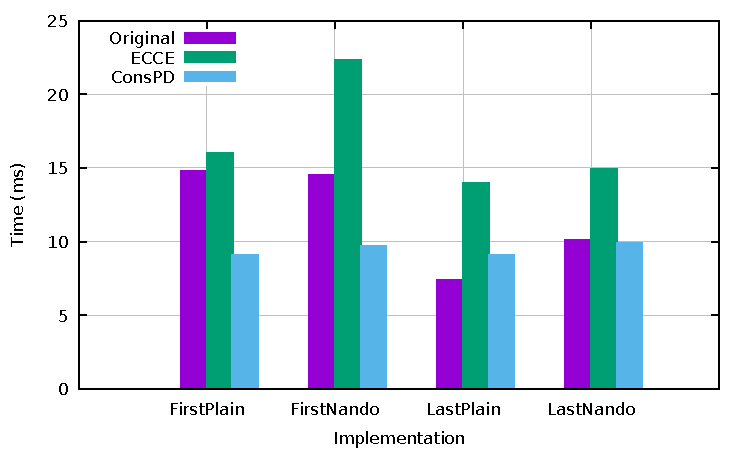
\includegraphics[width=\textwidth]{data/propEval/prop.pdf}
  \end{subfigure}
  \caption{Execution time of evalo}
  \label{fig:eval}
\end{figure}

Conservative partial deduction generates  programs with comparable performance for all four implementations, while the quality of \ecce specialization differs significantly.
\ecce worsens performance for every implementation as compared to the original program.
ConsPD do not worsen performance for any implementation.
Its effect is most significant for the implementations in which the boolean connectives are placed first within conjunctions.

\subsubsection{The Order of Answers}

It is important to note that different implementations of the same \mk relation produce answers in different orders.
Nevertheless, since \mk search is complete, all answers will be found eventually.
Unfortunately, it is not guaranteed that the first 1000 formulas generated with different implementations of \lstinline{eval$^o$} will be the same.
For example, $983$ formulas are the same among the first $1000$ formulas generated by the Original \emph{FirstPlain} relation and the same relation after the ConsPD transformation.
At the same time, only $405$ formulas are the same between the Original and \ecce \emph{LastNando} relations.

The reason why implementations differ so much in the order of the answers stems from the canonical search strategy employed in \mk.
Most \mk implementations employ \emph{interleaving} search~\cite{10.1145/1090189.1086390} which is left-biased.
It means that the leftmost disjunct in a relation is being executed longer than the disjunct on the right.
This property is not local which makes it very hard to estimate the performance of a given relation.

In practice it means that if a specializer reorders disjuncts, then the performance of relations after specialization may be unpredictable.
For example, by putting the disjuncts of the \lstinline{eval$^o$} relation in the opposite order, one produces a relation which runs much faster than the original, but it generates completely different formulas at the same time.
Most of the first 1000 formulas in this case are multiple negations of a variable, while the original relation produces more diverse set of answers.
Computing a negation of a formula only takes one recursive \lstinline{eval$^o$} call thus finding such answers is faster than conjunctions and disjunctions.
Meanwhile, the formulas generated by the reordered relation are less diverse and may be of less interest.

Although neither \ecce nor ConsPD reorder disjuncts, they remove disjuncts which cannot succeed.
Thus they influence the order of answers and performance of relations.
We believe that, in general, it is not possible to guarantee the same order of answers after specialization.
Exploring how different specializations influence the execution order is a fascinating direction for future research.


\subsection{Typechecker-Term Generator}

This relation implements a typechecker for a tiny expression language.
Being executed in the backward direction it serves as a generator of terms of the given type.
The abstract syntax of the language is presented below.
The variables are represented with de Bruijn indices, thus let-binding does not specify which variable is being bound.

\[\begin{array}{lllll}
  type \ term = &\ BConst \ of \ Bool &| \ IConst \ of \ Int &| \ Var \ of \ Int & \\
  & | \ term + term &| \ term * term &| \ term = term &| \ term < term \\
  &| \ \underline{let} \ term \ \underline{in} \ term
  &\multicolumn{2}{l}{| \ \underline{if} \ term \ \underline{then} \ term \ \underline{else} \ term} &
\end{array}\]

The typing rules are straightforward and are presented below.
Boolean and integer constants have the corresponding types regardless of the environment.
Only terms of type integer can be summed up, multiplied or compared by less-than operator.
Any terms of the same type can be checked for equality.
Addition and multiplication of two terms of suitable types have integer type, while comparisons have boolean type.
If-then-else expression typechecks only if its condition is of type boolean, while both then- and else-branches have the same type.
An environment $\Gamma$ is an ordered list, in which the $i$-th element is the type of the variable with the $i$-th de Bruijn index.
To typecheck a let-binding, first, the term being bound is typechecked and is added in the beginning of the environment $\Gamma$, and then the body is typechecked in the context of the new environment.
Typechecking a variable with the index $i$ boils down to getting an $i$-th element of the list.

\begin{table}[!h]
  \setlength{\tabcolsep}{0.4cm}
  \centering
  \begin{tabular}{c c c}
    \infer[]{\Gamma \vdash IConst \ i : Int}{} &
    \infer[]{\Gamma \vdash BConst \ b : Bool}{}  &
    \infer[\Gamma \lbrack v \rbrack \equiv \tau]{\Gamma \vdash Var \ v : \tau}{} \vspace{0.5cm}
    \\
    \infer[]{\Gamma \vdash t + s : Int}{\Gamma \vdash t : Int, \Gamma \vdash  s : Int}  \vspace{0.5cm} &
    \infer[]{\Gamma \vdash t = s : Bool}{\Gamma \vdash t : \tau, \Gamma \vdash  s : \tau} &
    \infer[]{\Gamma \vdash \underline{let} \ v \ b : \tau}{\Gamma \vdash v : \tau_v, \ (\tau_v :: \Gamma) \vdash b : \tau}
      \\

      \infer[]{\Gamma \vdash t * s : Int}{\Gamma \vdash t : Int, \Gamma \vdash  s : Int}  &
    \infer[]{\Gamma \vdash t < s : Bool}{\Gamma \vdash t : Int, \Gamma \vdash  s : Int} \vspace{0.5cm} &
      \infer[]{\Gamma \vdash \underline{if} \ c \ \underline{then} \ t \ \underline{else} \ s : \tau}{\Gamma \vdash c : Bool, \Gamma \vdash t : \tau, \Gamma \vdash s : \tau}
  \end{tabular}
\end{table}


We compared two implementations of these typing rules.
The first one is obtained by unnesting of a functional program as described in~\cite{lozov2019relational} (\emph{Generated}).
It is worth noting that the unnesting introduces a lot of redundancy in form of extra unifications and thus creates programs which are very inefficient.
Thus we contrast this implementation with the program hand-written in \oc (\emph{Hand-written}).
Each implementation has been specialized with ConsPD and \ecce.
We measured the time needed to generate 1000 closed terms of type integer (see Fig.~\ref{tbl:type}).


\begin{figure}[!h]
  \begin{subfigure}[c]{0.55\textwidth}
    \centering
    \begin{tabular}{c||c|c|c}
                          & Original & \ecce & ConsPD  \\ \hline\hline
      \emph{Hand-written} & 0.92s    & 0.22s & 0.34s   \\ \hline
      \emph{Generated}    & 11.46s   & 0.38s & 0.29s
      \end{tabular}
  \end{subfigure}
  \hfill
  \begin{subfigure}[c]{0.45\textwidth}
    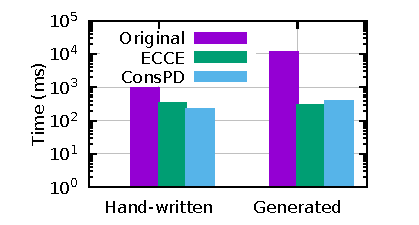
\includegraphics[width=\textwidth]{data/lTypecheck/ltypelog.pdf}
  \end{subfigure}
  \caption{Execution  time of generating 1000 closed terms of type Integer}
  \label{tbl:type}
\end{figure}

As expected, the generated program is far slower than the hand-written.
The principal difference between these two implementations is that the generated program contains a certain redundancy introduced by unnesting.
For example, typechecking of the sum of two terms in the hand-written implementation consists of a single conjunction (see Listing~\ref{type:hand}) while the generated program is far more complicated and also uses a special relation \lstinline{typeEq$^o$} to compare types (see Listing~\ref{type:gen}).

\begin{figure*}[!h]
  \centering
    \begin{lstlisting}[label={type:hand}, caption={A fragment of hand-written typechecker}, captionpos=b, frame=tb]
  let rec typecheck$^o$ gamma term res = conde [
    ...
    fresh (x y) ((term === x + y /\
       typecheck$^o$ gamma x ^(Some Integer) /\
       typecheck$^o$ gamma y ^(Some Integer) /\
       res === ^(Some Integer)));
    ...]
    \end{lstlisting}
\end{figure*}


\begin{figure*}[!t]
  \centering
    \begin{lstlisting}[label={type:gen}, caption={A fragment of generated typechecker}, captionpos=b, frame=tb]
let rec typecheck$^o$ gamma term res = conde [
  ...
  fresh (x y t1 t2) ((term === x + y /\
    conde [
      typecheck$^o$ gamma x ^None       /\ res === ^None;
      typecheck$^o$ gamma x ^(Some t1) /\
        typecheck$^o$ gamma y ^None     /\ res === ^None;
      typecheck$^o$ gamma x ^(Some t1) /\  typecheck$^o$ gamma y ^(Some t2) /\
        typeEq$^o$ t1 Integer ^true     /\ typeEq$^o$ t2 Integer ^true /\
        res === ^(Some Integer);
    ])
  ...]
    \end{lstlisting}
\end{figure*}

Most of the redundancy of the generated program is removed by specialization with respect to the known type of the term.
This is why both implementations have comparable speed after specialization.
\ecce shows bigger speedup for the hand-written program than ConsPD and vice versa for the generated implementation.
We believe that this difference can be explained by too much unfolding.
\ecce performs a lot of excessive unfolding for the generated program and only barely changes the hand-written program.
At the same time ConsPD specializes both implementations to comparable programs performing average amount of unfolding.
This shows that the heuristics we presented gives more stable, although not the best, results.

% У заключения нет номера главы
\clearpage

\section*{Заключение}
В ходе данной работы получены следующие результаты. 
\begin{itemize}
  \item Изучена предметная область: методы обработки встроенных языков и алгоритм обобщённого синтаксического анализа RNGLR.
  \item Разработан алгоритм синтаксического анализа динамически формируемых выражений, поддерживающий работу с произвольными входными графами.
  \item Доказана корректность алгоритма:
  \begin{itemize}
    \item алгоритм завершит работу для любых входных данных;
          %для любой входной детерминированной контекстно-свободной грамматики и 
          %произвольного входного графа алгоритм завершит свою работу;
    \item для любой цепочки из входного множества, выводимой в эталонной грамматике G, в SPPF содержится её дерево вывода в G; при этом никакие другие деревья не содержатся в SPPF.
          %для любой цепочки, которую может породить автомат (которая содержится 
          %в регулярном множестве), выводимой в рассматриваемой грамматике G, в 
          %SPPF содержится её дерево вывода в G, при этом не содержится никаких 
          %других деревьев.
  \end{itemize}
  \item Выполнена реализация алгоритма на языке программирования F\# в рамках исследовательского проекта YaccConstructor.
  \item Проведена апробация: регрессионное тестирование, тестирование производительности и тестирование на реальных данных.
  \item Исходный код проекта YaccConstructor можно найти на сайте \url{https://github.com/YaccConstructor/YaccConstructor}, автор принимал участие под учётной записью kajigor.
\end{itemize}

В дальнейшем планируется изменить алгоритм таким образом, чтобы помимо 
построения леса разбора всех корректных выражений осуществлялся бы также поиск ошибочных выражений и сообщение о них. Также необходимо произвести теоретическую оценку сложности алгоритма. Предложенный алгоритм планируется внедрить в инструмент по реинжинирингу информационных систем.  

\section*{Acknowledgments}

The research was supported by the Russian Science Foundation grant 18-11-00100 and a grant from JetBrains Research.

\bibliographystyle{ACM-Reference-Format}
\bibliography{combinators_for_graph_querying}

\end{document}
